\documentclass{article}

% if you need to pass options to natbib, use, e.g.:
% \PassOptionsToPackage{numbers, compress}{natbib}
% before loading nips_2016
%
% to avoid loading the natbib package, add option nonatbib:
% \usepackage[nonatbib]{nips_2016}

\usepackage[final]{nips_2016}

% to compile a camera-ready version, add the [final] option, e.g.:
% \usepackage[final]{nips_2016}

\usepackage[utf8]{inputenc} % allow utf-8 input
\usepackage[T1]{fontenc}    % use 8-bit T1 fonts
\usepackage{hyperref}       % hyperlinks
\usepackage{url}            % simple URL typesetting
\usepackage{booktabs}       % professional-quality tables
\usepackage{amsfonts}       % blackboard math symbols
\usepackage{nicefrac}       % compact symbols for 1/2, etc.
\usepackage{microtype}      % microtypography
\usepackage{listings}
\usepackage{graphicx}

\graphicspath{{./figures/}}

\title{CS380L Project Writeup: Distributed Completion Service}

% The \author macro works with any number of authors. There are two
% commands used to separate the names and addresses of multiple
% authors: \And and \AND.
%
% Using \And between authors leaves it to LaTeX to determine where to
% break the lines. Using \AND forces a line break at that point. So,
% if LaTeX puts 3 of 4 authors names on the first line, and the last
% on the second line, try using \AND instead of \And before the third
% author name.

\author{
  Jason Z. Liang \\
  Department of Computer Science\\
  University of Texas at Austin \\
  \texttt{jasonzliang@utexas.edu} \\
}

\begin{document}

\maketitle

\begin{abstract}
  Task parallelism is difficult to implement in a distributed setting due to machine unreliability and communication latency. HTCondor, an existing distributed computation framework, is insufficient for addressing these shortcomings. In this report, we present a high level abstraction built on top of HTCondor called the Distributed Completion Service (DCS). The DCS uses multiple different methods to improve upon reliability and latency. Experiment results reveal DCS's ability to scale and demonstrate a reduction in latency when compared to just using HTCondor alone.
\end{abstract}

\section{Introduction and Background}

Task parallelism, especially in a distributed setting where multiple tasks are running concurrently on a separate machines, has been an area of intense research recently. Tasks parallelism is useful tool for solving computationally heavy problems in many areas of computer science. For example, in deep learning, it is often leveraged to perform hyperparameter search concurrently on many different neural network models \cite{bergstra2013hyperopt}. It is also used to support essential web services such as web search and indexing \cite{boldi2004ubicrawler}. However, distributed task parallelism is considered to be a challenging problem due to the following reasons: 1) Hardware and software are unreliable and nodes/tasks may fail or become unavailable at any moment. 2) A small fraction of tasks sometimes can lag behind the rest (also know as the straggler problem). 3) There might be high communication and startup latency for the worker nodes. 4) Implementing a distributed algorithm often requires writing a lot of boiler plate code.

Many distributed frameworks have tried to alleviate these issues and maximize the throughput of a computational cluster; these include Map Reduce \cite{dean2008mapreduce}, Spark \cite{zaharia2010spark}, and Dandelion \cite{rossbach2013dandelion}. Most of these frameworks contain sophisticated algorithms that increase system reliability and minimize the performance cost and latency of executing tasks. The distributed framework in the UTCS Department, HTCondor \cite{thain2005distributed}, solves some of the low level issues associated with distributed computing such as job scheduling and user multiplexing; however it is not capable of solving the problems stated above. HTCondor incurs high latency between the submission of jobs and their execution and furthermore, it has no reliability guarantees for successful completion of tasks. Lastly, submitting jobs to HTCondor requires creating a verbose submission file with many flags and options that are irrelevant to many users.

This report presents a novel distributed framework built on top of HTCondor called the Distributed Completion Service (DCS). At its core, the DCS is a service which decouples the production of new asynchronous tasks from the consumption of the results of completed tasks. It provides improved reliability against task failure, a method to detect and handle stragglers, reduced latency and overhead, and a simple clean API for users.

\section{Distributed Completion Service Design Overview}

The DCS is composed of four main components: 1) A server that represents an entry point for the user to submit tasks and get back results. 2) Clients that run either locally on the same machine as the server or on remote machines through HTCondor. 3) A client manager which allows the user to control the number of clients running locally and on HTCondor. 4) A pair of submit and return queues which is used to send tasks from the server to the client and results from the client back to the server.

The typical workflow for an user utilizing the DCS would be as follows: 1) The manager is used to spin up a fixed number of clients either locally or HTCondor. 2) The user submits tasks through the server, which the server then pushes into the submit queue. Running clients pull tasks from the submit queue in the order in which the tasks are submitted (FIFO) and begin working on them. Once the task is finished, the standard output of the task is placed onto the result queue. The server will then pull the results from that queue and return them back to the user. Exit codes are also passed back to the user as part of the results and are used to indicate whether the task is successfully executed or not (non zero exit code means failure).

\subsection{User API}

The API for the DCS has been explicitly designed to be easy to use. As such, there are only two main functions which the user can call. They are the following:

\begin{lstlisting}[language=Python]
submitTask(task, task_data, estimated_time)
getResults(timeout)
\end{lstlisting}

In submitTask(), the user provides a string that points to the filesystem path of a shell runnable script or program (task), a list of arguments to the task (task\_data), and optionally an estimate of how long the task will take (estimated\_time). The getResults() function takes a single argument (timeout) that specifies how long getResults() should block for while waiting on the result queue for the result of a submitted task to arrive. If a result is not returned before exceeding the timeout, a null reference is returned instead. Below is an example of how the user would use these two functions to perform computation in parallel.

\begin{lstlisting}[language=Python]
x = CompletionServiceServer(clean_start=True)
for i in xrange(100):
  x.submitTask("test_tasks/square.py", i)
for i in xrange(100):
  print "i:", x.getResults().task_data
\end{lstlisting}

As the example above shows, the user can easily leverage massive task parallelism in only 5 lines of code. This is much less than the amount of boilerplate code needed to execute the same tasks using HTCondor.

\subsection{Reliability}

Unlike HTCondor, which provides no guarantee for successful completion of tasks, DCS improves reliability by allowing each task to be retried by the client up to $K$ times, where $K>1$ is a hyperparameter specified by the user (by default it is set to 3). Alternatively, if there are $K$ more idle clients (clients not working on a task) than the number of tasks in the submit queue, the computer service will submit $K$ copies of the same task.

This policy guarantees that the user will have a high chance of getting a successful result for the task within bounded time. The probability of task failure decreases exponentially as $K$ increases. Assuming each task has $C$ chance of failure where $0<C<1$, the chance of getting at least once successful result back for a task is $1-C^K$; as we see converges quickly to 1. In the worse case, the amount of time to get back all results for the tasks bounded by $K*(TM/C)$, where $T$ is the number of tasks, $K$ the number of clients, $M$ the time of the longest task, and $C$ is the number of clients available. In the best case, when $C>>T$, overall running time is $TM/C$. This time is no different than if each task is completely reliable and no retries are required. Thus in the worse case scenario, the overall running time when trying unreliable tasks is only $K$ times longer than completely reliable tasks.

\subsection{Detecting and Handling Stragglers}

Straggler handling is another important shortcoming of HTCondor that the DCS deals with. Stragglers are tasks which complete much slower than expected due to the slow performance of the hardware on which the client is running on, or the client being frequently suspended by the HTCondor job manager. To deal with stragglers, DCS will automatically estimate the running time of all tasks submitted. To do so, it will keep a history of the running times of all past tasks that returned results. When submitting a new task, its running time is conservatively estimated as the the mean running time plus two standard deviations of the past running times. If the actual running time of the task is $P$ ($P>1$ and set to 2 by default) times longer than the estimated running time, the task is deemed a straggler.

Straggling tasks are allowed to complete on their current client, however they are also moved back into the submit queue. There, another client can pull the straggling task and work on it. Straggling tasks can only be restarted a limited number of times. The number of times a task can be retried due to failure or flagged as straggling cannot exceed a total of $K$ times. This ensures that the system will not wait indefinitely for an straggling task to finish.

\subsection{Minimizing Task Latency}

Compared to HTCondor, the DCS exhibits much lower latency for the submission/execution of tasks when all the clients are running. This is due to DCS avoiding the overhead of the HTCondor job scheduler, which depending on the overall system load, can add at least 30 seconds to several minutes of delay before jobs begin running. When using the DCS with clients running locally on the same machine equipped with a SSD, the latency between submitting a task and having the task begin execution can be as few as several milliseconds. When on a machine with network file system (NFS) \cite{sandberg1985design} and clients running on HTCondor, the latency is usually only around several hundred milliseconds. However, if the user tries submit tasks to the DCS from a cold start (with no clients running), the user will still incur the heavy initial penalty of starting up clients on HTCondor.

To remedy this issue, DCS has an ability to running in a setting called "hybrid mode". In "hybrid mode", DCS will not only spin up clients locally, but on HTCondor as well. The clients on HTCondor will still pull tasks in a FIFO manner, but the local clients will prioritize pulling tasks from the submit queue that have shortest estimated running times. This allows short tasks to be executed and completed even before the clients on HTCondor are up and running. If the user is submitting a significant fraction of tasks that complete quickly, the fast completion of these tasks can help mask the startup latency incurred by running clients on HTCondor.

\section{Implementation Details and Tricks}

The DCS is implemented in Python \cite{van2007python} using mostly standard library modules. Python is chosen because its powerful standard library contains useful components for performing filesystem traversal, object serialization/deserialization, and managing/forking processes. Some preliminary benchmarking and profiling has shown that the performance bottleneck is usually due to filesystem reads and writes. Thus, Python is considered to be sufficiently fast enough as the language for the first version of the DCS.

When the DCS server starts up, it creates a base directory. This base directory contains the working directories of the server and clients. When the clients or server pulls tasks from the queues, these tasks are stored in their respective working directories. The working directories also contain log files and can be used to debug crashed remote clients.

\subsection{Container Object for Tasks and Results}

Submitted task and returned results are encapsulated into a container object before they are serialized and placed into a queue. Serialization and deserialization of the object is performed using the cPickle standard library module. Pickle files are binary encodings of arbitrary Python objects and do not require a schema or writing any additional code. An explanation of the fields of the container object is provided below:

\begin{enumerate}
\item \textbf{time\_created}: time when task or result is created.
\item \textbf{uid}: random string that is the same for duplicate submitted tasks, retried tasks, and submitted task/result pairs.
\item \textbf{num\_failures}: number of times that the task has failed and been retried.
\item \textbf{is\_result}: boolean flag whether object contains a result or submitted task.
\item \textbf{task}: a filepath string of the command/program to run if object contains a submitted task, otherwise None.
\item \textbf{task\_data}: a string of command arguments for submitted tasks, otherwise output result of submitted task.
\item \textbf{estimated\_time}: estimated time for submitted task, otherwise None.
\item \textbf{metadata}: for object containing result, this is a dictionary with information about a completed task such as exit code, time elapsed, and standard error.
\end{enumerate}

\subsection{Submit and Return Queues}

The submit and return queues are both filesystem based queues which allow atomic push() and pop() operations without the use of locks. Each queue is represented as a directory and tasks/results in the queues are represented as files inside the directory. Each task has a unique filename that is composed of a random string, the time when it is added to the queue, and the estimated time of the task. These information are included as part of the filename in order to simplify lookup when pulling tasks from the queue based on either earliest timestamp, or shortest estimated running time.

The queues must be safe from race conditions even if the server and multiple clients are simultaneously using the queue at the same time. To ensure good performance of the push() and pop() operations, no locking is used for the queues. Instead, the push() operation is ensured to be atomic by using the rename() system call, which is guaranteed to atomic on all POSIX compliant filesystems, including NFS. The task is first serialized to a temporary file and then moved using rename() into the queue directory. Similarly, when popping tasks from a queue, the task is moved into the working directory of the client or server and then deserialized.

It is interesting to note that non-filesystem system queues are also considered when designing the DCS. For example, the shared queue between clients and server could be implemented as a another server where all the clients and the first server connect to it through network sockets. The tasks on the queue server would be stored in memory and accessed through a multiple producer, multiple consumer thread-safe queue. However, because the performance of the NFS filesystem is sufficiently high and due to the complexity of implementing a protocol for communicating through the network, a filesystem based queue is chosen instead.

\subsection{Client Heartbeat and Command Files}

One issue with running clients on HTCondor is that their reliability are not guaranteed. The HTCondor job scheduler can kill or suspend clients at any moment without warning. Thus, one of the necessary duties of the server is to detect clients which failed and move any incomplete tasks of the failed clients back into the submit queue. This is achieved by having the clients maintain a heartbeat file in their working directory. Every $H$ seconds, the client must refresh the heartbeat file with the current time. The server checks the heartbeat files of all the clients at regular intervals. If a heartbeat file is more than $I * H$ seconds old, then the client is deemed to have failed, and the server can proceed with cleanup. By default, $I=5$ and $H=3$.

Client also constantly scan for the presence of a command file in their working directory. If it detects a command file, it will open it and execute the commands inside. The currently supported commands are the following: 1) finish the current task and then shutdown and 2) shutdown immediately. The command file is used by the manager to shutdown clients and is much simpler than keeping track of PIDs of local clients and the job IDs of HTCondor clients. Clients also automatically shutdown if their working folder is deleted.

\begin{figure}[t]
  \begin{center}
    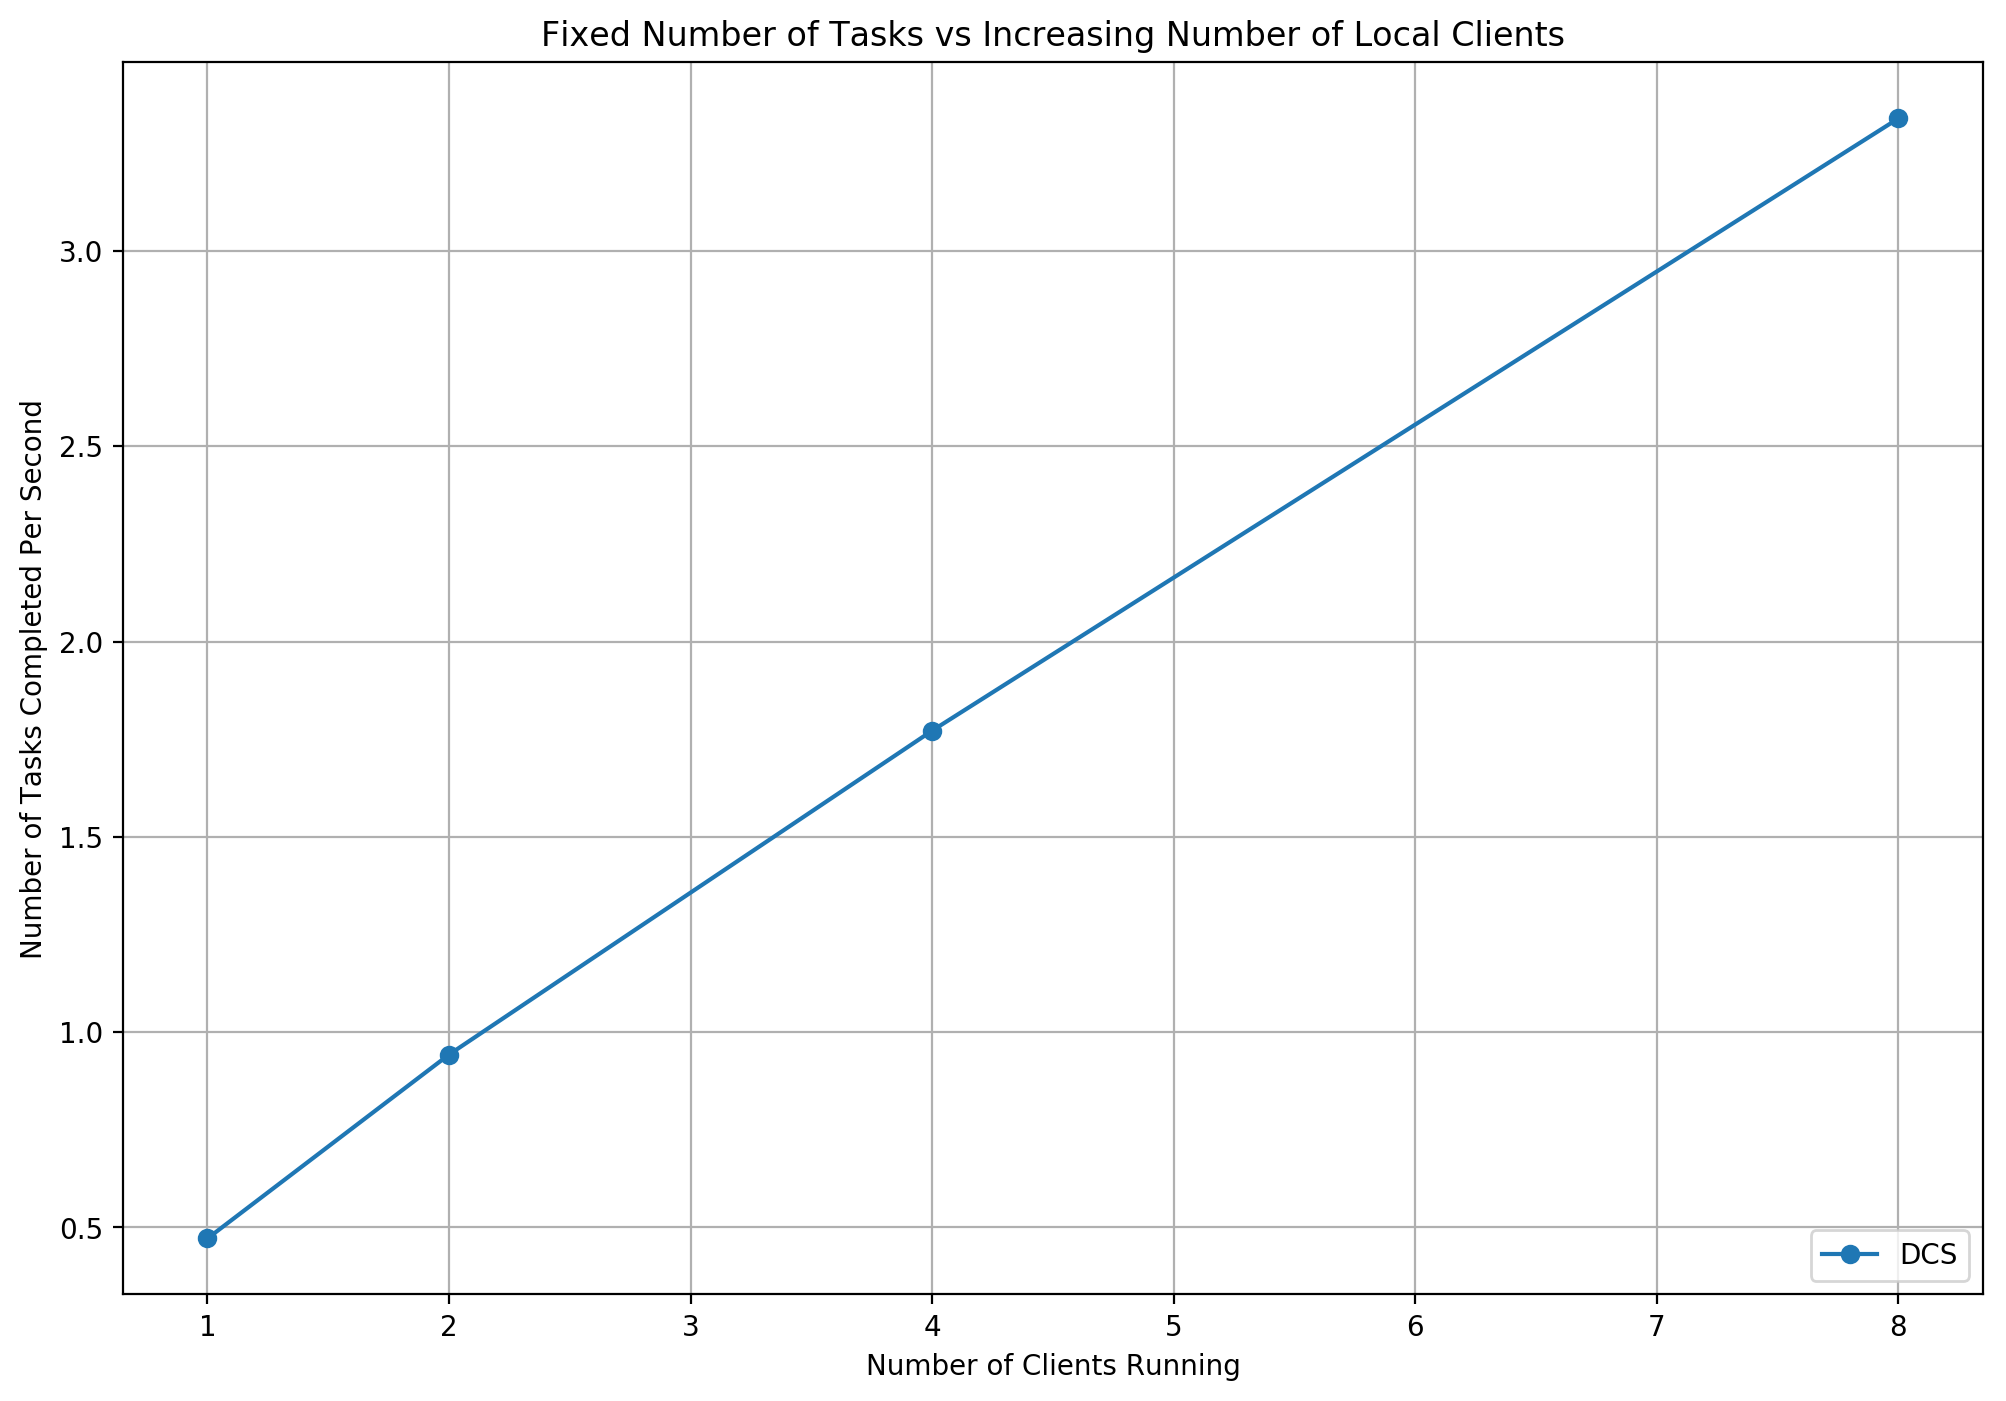
\includegraphics[width=0.4\textwidth]{client_scaling_local.png}
    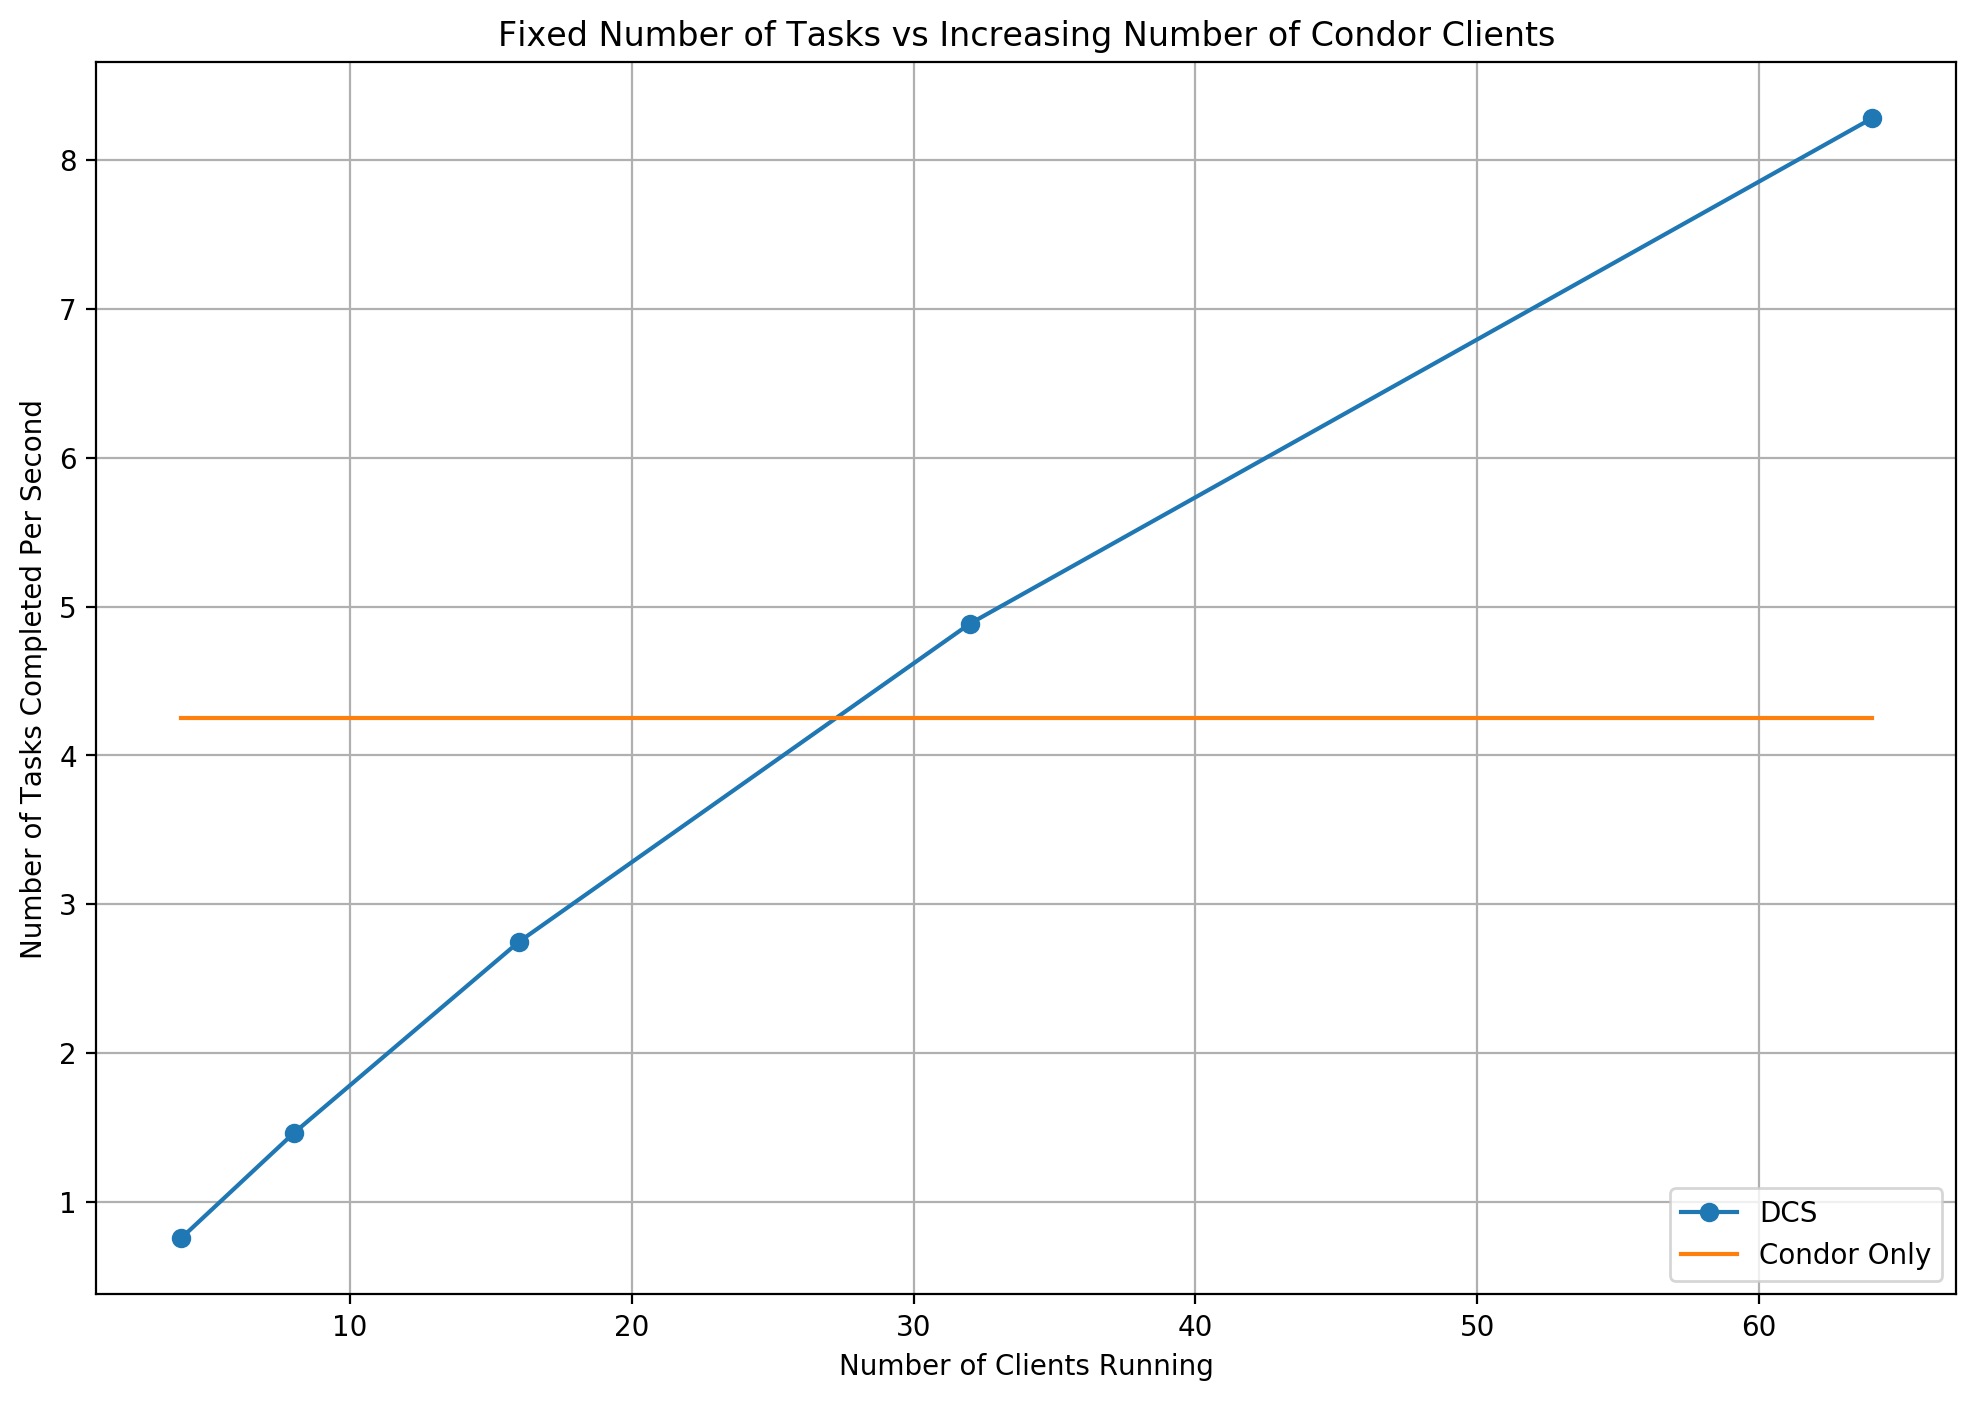
\includegraphics[width=0.4\textwidth]{client_scaling_condor.png}
    \caption{Left: Plot shows how task throughput increases with the number of local clients. Right: Plot shows how task throughput increases with the number of HTCondor clients. The orange line shows task throughput when submitting 128 tasks directly through HTCondor. Both plots show mean values from 5 trials.}
    \label{fg:client_scaling}
  \end{center}
\end{figure}

\section{Experimental Results}

All of the experiments are run on a UTCS instructional machine with 8 cores, 16 GB of ram, and NFS filesystem. The machine is also connected to HTCondor and can submit up to 150 jobs at a time. All of the experimental plots show mean results from 5 trials. Because the variance between each trial is not very large, standard error bars are omitted for the sake of clarity.

\subsection{Scaling vs Number of Running Clients}

In the first experiment, we examine how DCS scales with increasing number of local and HTCondor clients. First we examine task throughput of DCS (defined as number of tasks finished per second) when we increase the number of local clients. We submit 64 tasks (each task taking 2 seconds to finish) with 1, 2, 4, and 8 local clients running. The left plot in Fig.~\ref{fg:client_scaling} shows that task throughput increases nearly linearly; this is good news as it indicates adding more clients strongly improves performance. Next, we take a look at throughput with clients running on HTCondor. We submit 128 tasks (each task taking around 5 seconds) with 4, 8, 16, 32, and 64 HTCondor clients running. The right plot in Fig.~\ref{fg:client_scaling} shows very similar results, with throughput increasing almost linearly as well. For comparison sakes, we also show the task throughput when we submit all 128 tasks directly through HTCondor without DCS and have then all be executed simultaneously. As we can see, the task throughput when only using HTCondor is exceeded by DCS with just 32 clients. This is caused by the delay and overhead when starting jobs on HTCondor.

\begin{figure}[t]
  \begin{center}
    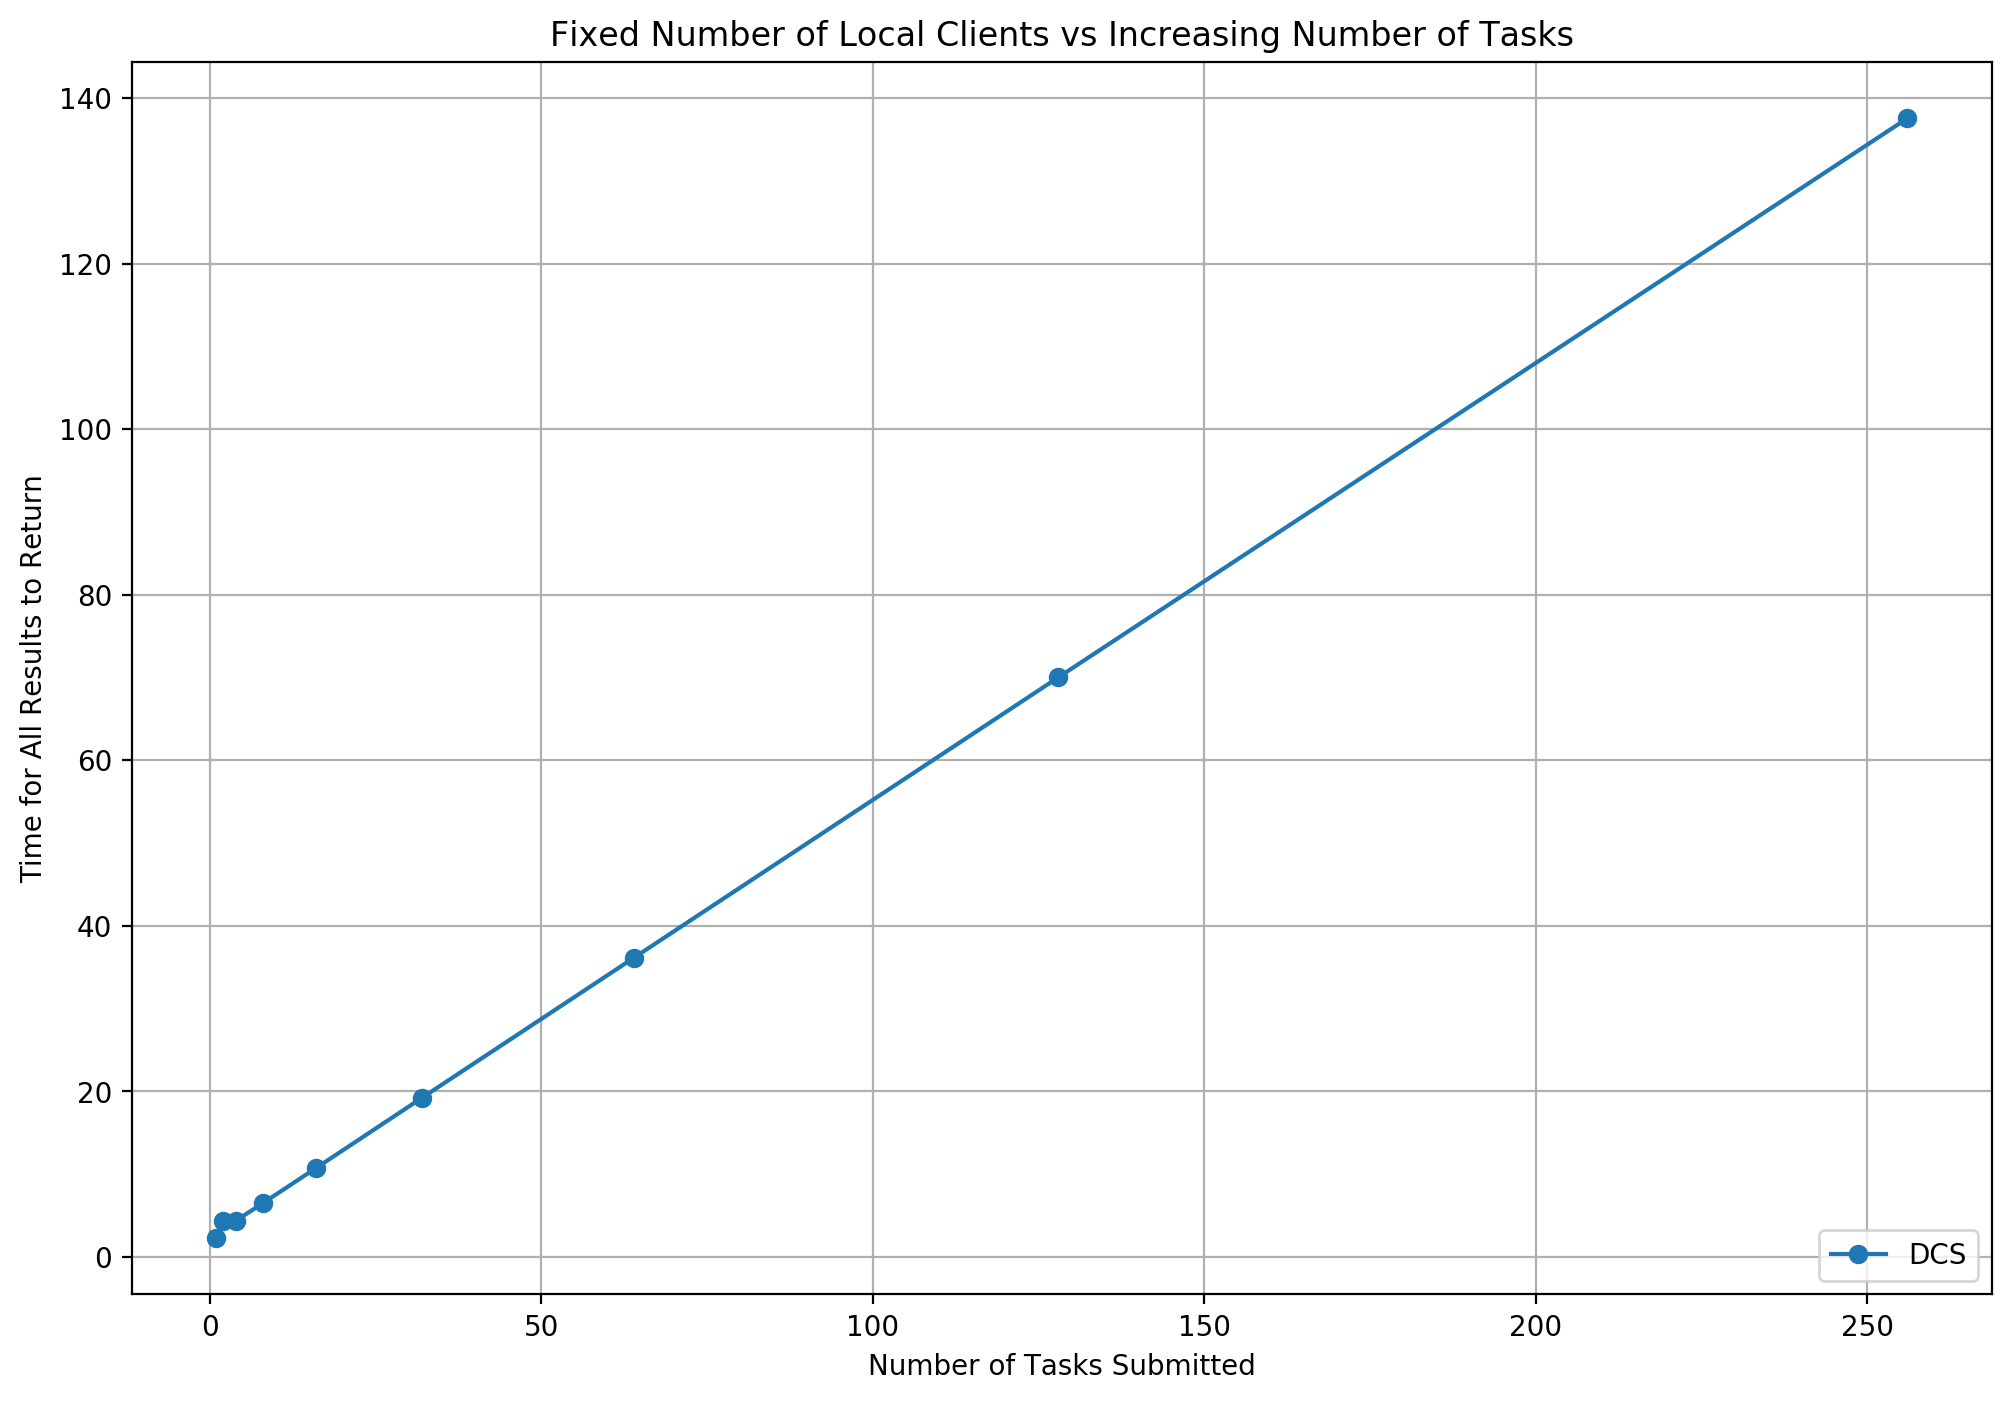
\includegraphics[width=0.4\textwidth]{task_scaling_local.png}
    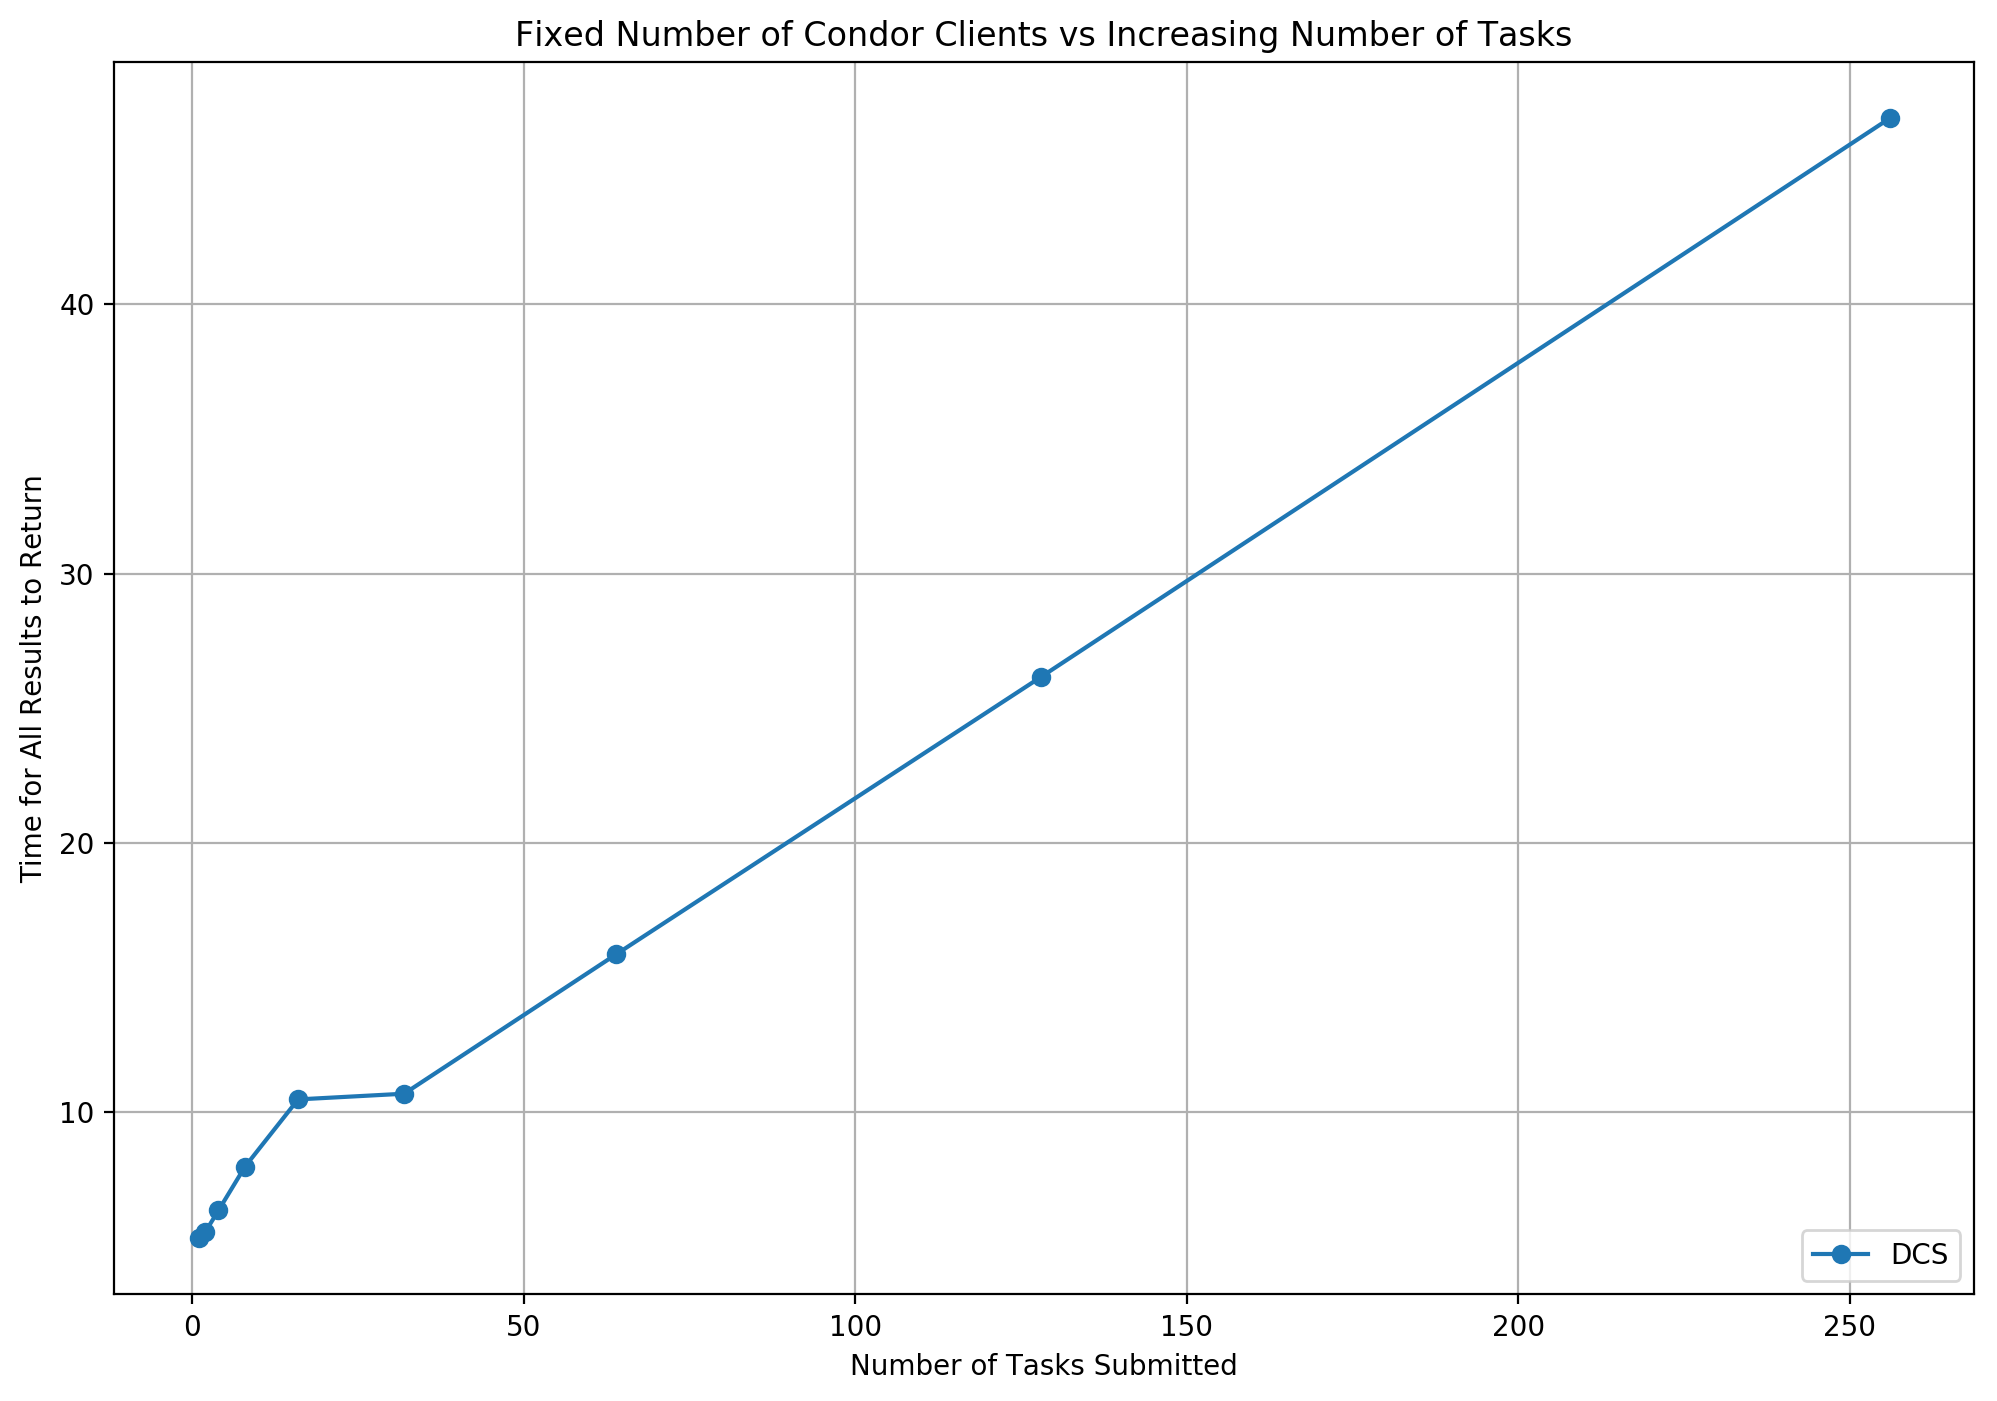
\includegraphics[width=0.4\textwidth]{task_scaling_condor.png}
    \caption{These two plots showing how total time to get back all results increases with number of tasks. Left: 4 local clients. Right: 32 HTCondor clients. Both plots show mean values from 5 trials.}
    \label{fg:task_scaling}
  \end{center}
\end{figure}

\subsection{Scaling vs Number of Tasks}

In our second experiment, we take a look at how running time of DCS increases when the number of running clients is fixed and the number of tasks submitted increases. In the left plot of Fig.~\ref{fg:task_scaling}, we submit anywhere from 1 to 256 tasks (each task taking 2 seconds to complete) with 4 local clients running. In the right plot of Fig.~\ref{fg:task_scaling}, we submit anywhere from 1 to 256 tasks (each task taking 5 seconds) with 32 HTCondor clients running. In both cases, the scaling is highly linear when the number of tasks submitted exceed the number of clients running. When the number of tasks is less than the number of clients, the total time it takes to finish all the tasks is much more noisy. This is probably due to the fact that we summit duplicates of the same task as part of the DCS's policy to improve reliability.

\subsection{Success Rate vs Number of Retries}

Finally, in our third experiment, we examine how the task success rate (defined as at least one successful result for a task) increases as the number of retries $K$ increases as well. We submit 500 tasks where each task has a 50 percent chance of failure and exits immediately with 4 clients running locally. The left plot of Fig.~\ref{fg:success_rate} shows that the actual success rate (blue line) is very much in line with the theoretical success rate (orange line) calculated earlier. Interestingly enough, the right plot shows the overall running time does not increase linearly with the number of retries. This is probably because most tasks do not need the maximum number of retries to achieve success and thus, only a small fraction of the tasks would suffer the worst case scenario.

\begin{figure}[t]
  \begin{center}
    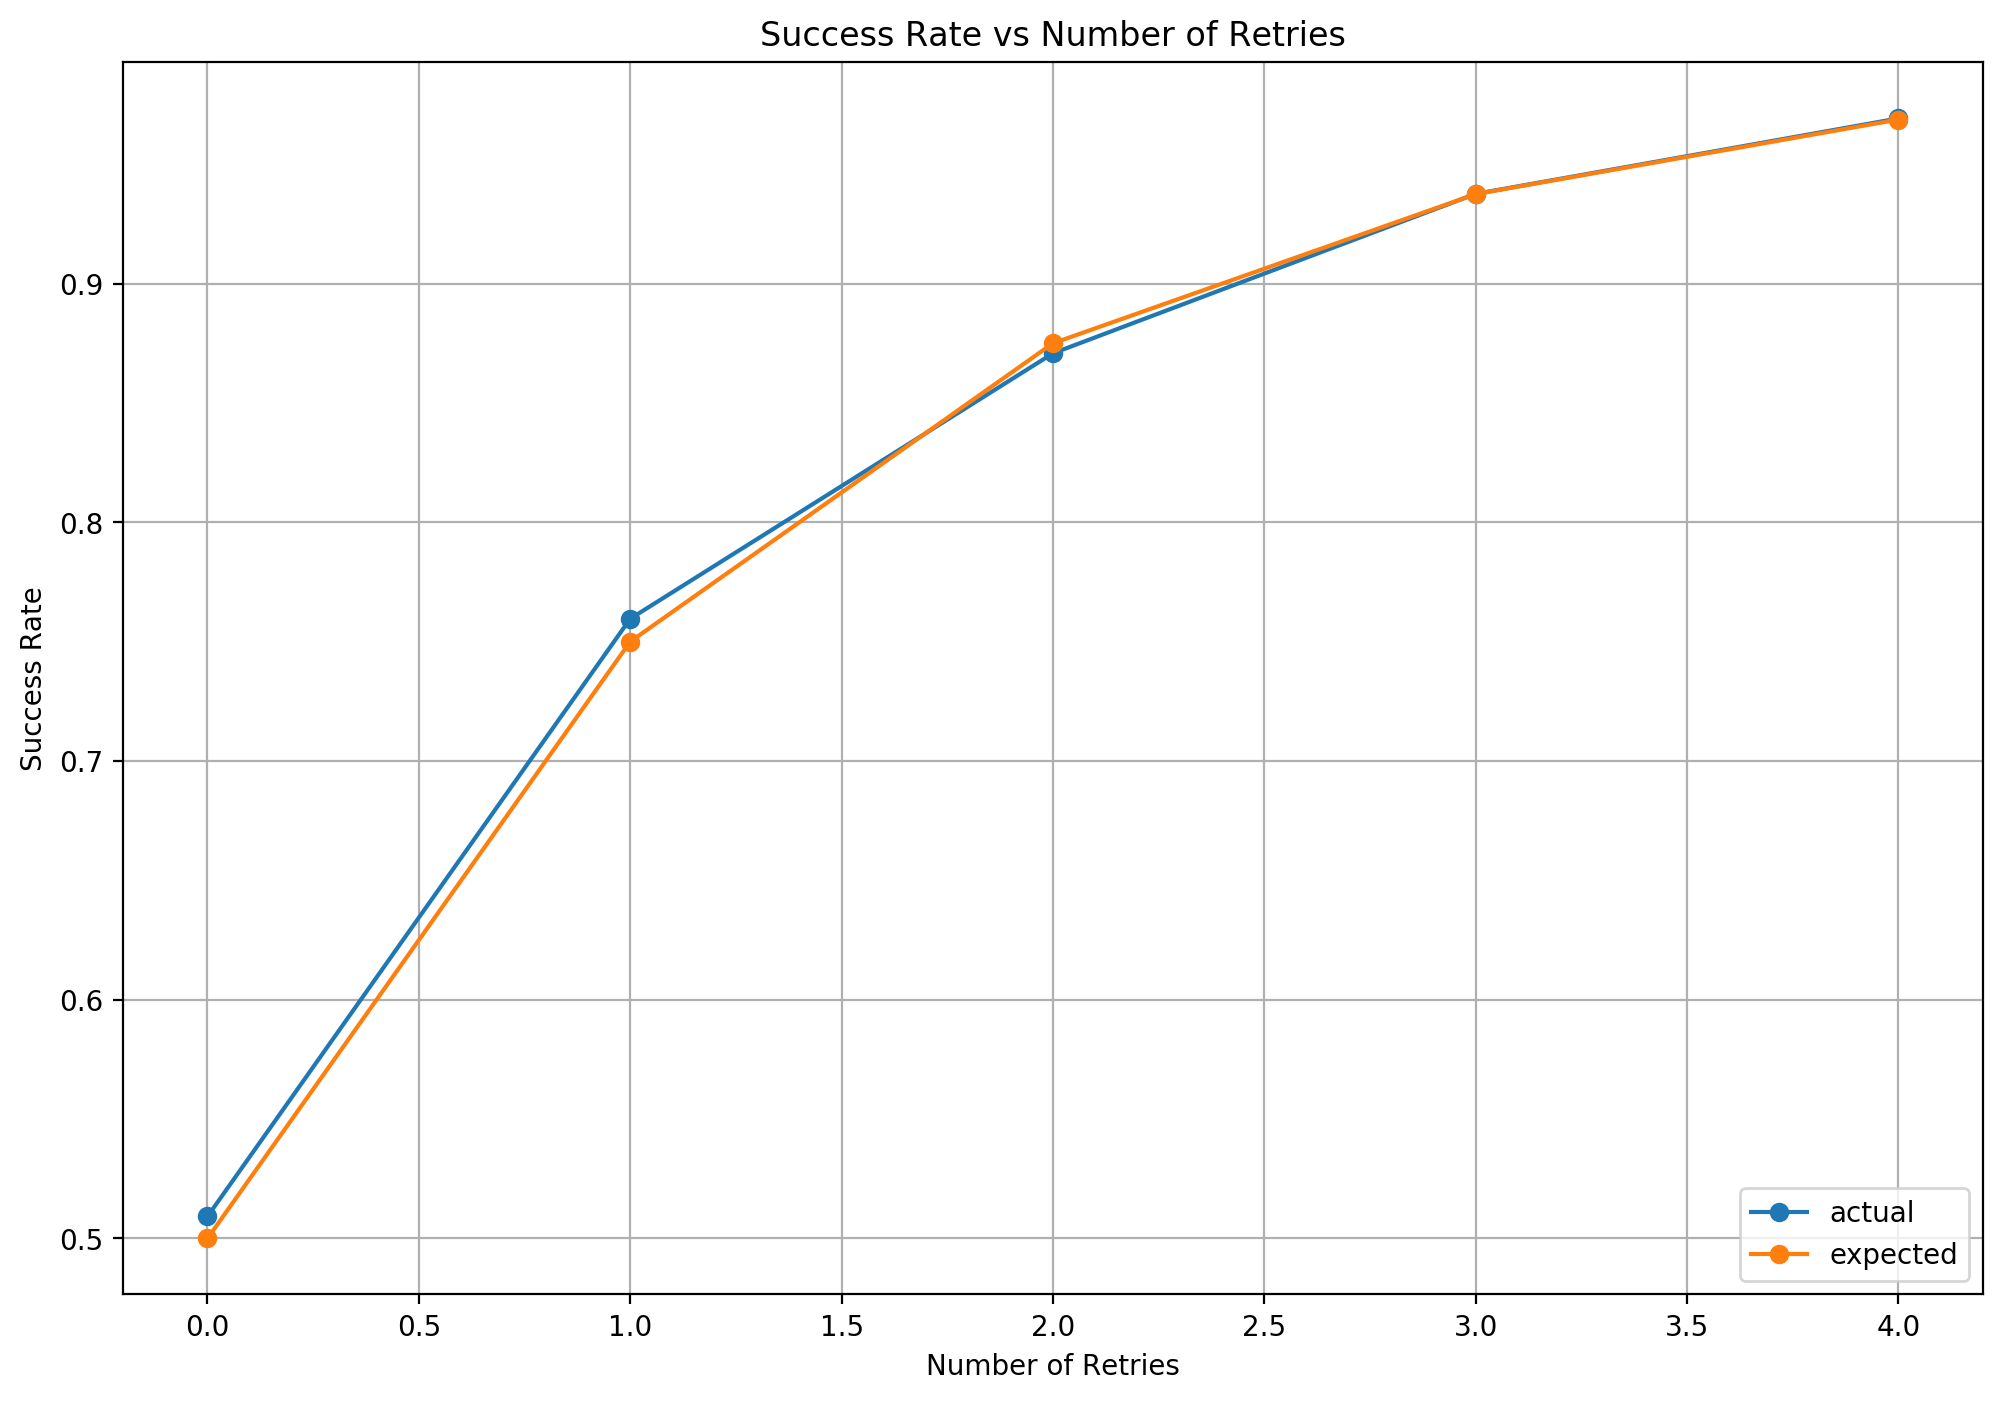
\includegraphics[width=0.4\textwidth]{succ_rate_task_error_local.png}
    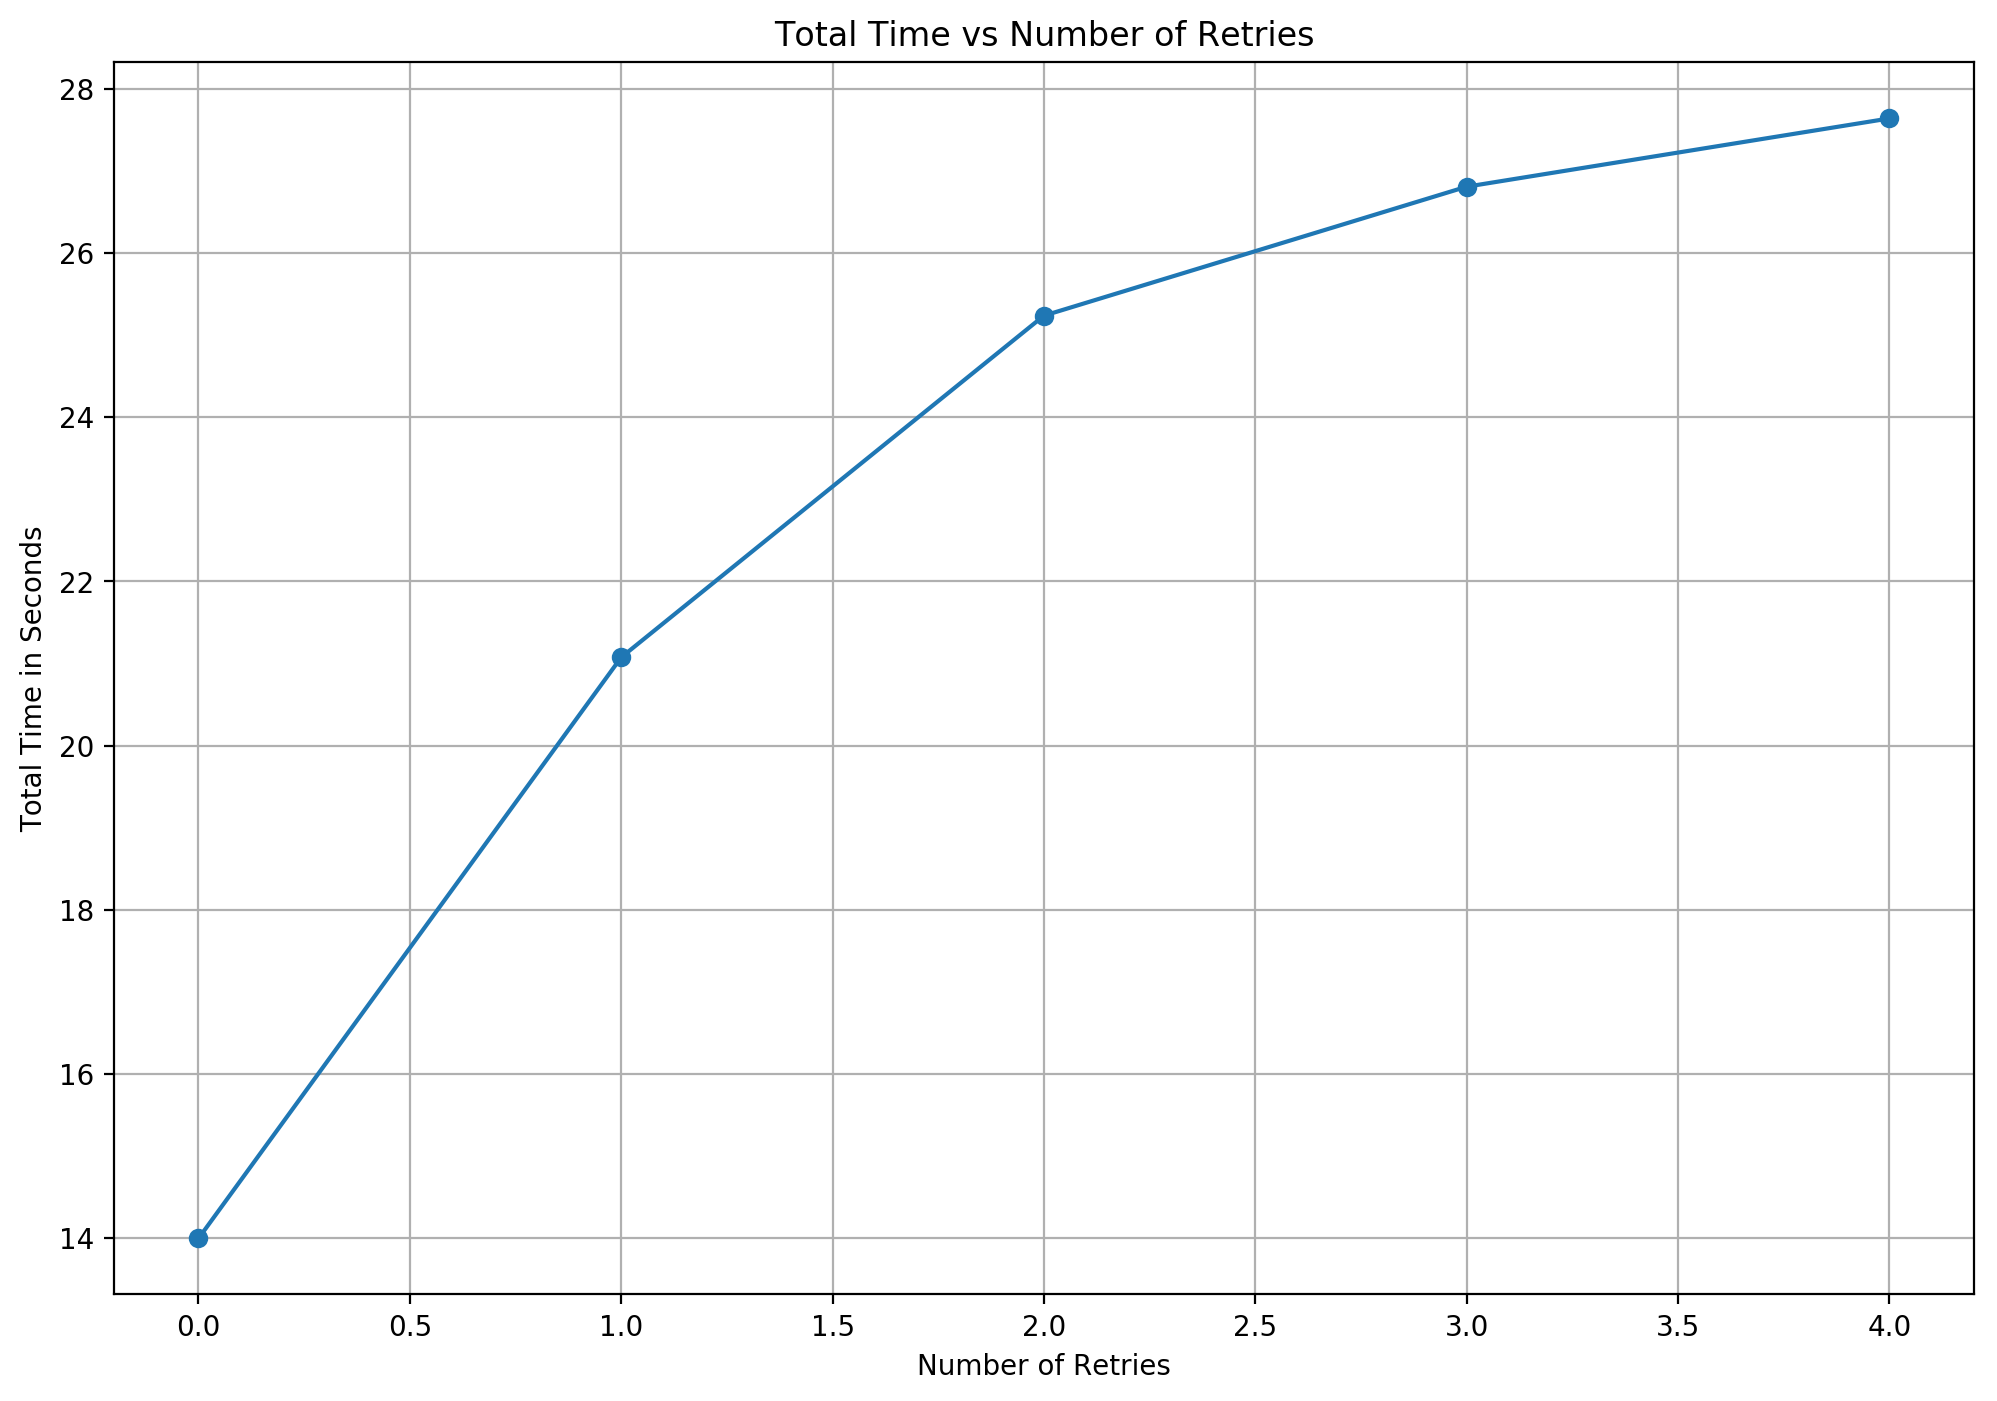
\includegraphics[width=0.4\textwidth]{timing_task_error_local.png}
    \caption{Left: Plot shows hows success rate increases as the number of retries increases. Right: Plot shows the total time to get back all results vs the number of retries. Both plots show mean values from 5 trials.}
    \label{fg:success_rate}
  \end{center}
\end{figure}

\section{Limitations and Future Work}

As this is the first version of the DCS, there are several inherent limitations due to how it is built on top of HTCondor. For example, there are no real way to prevent clients from being killed or suspended by the HTCondor job scheduler. Similarly, depending on the system load and priority of the current user, the clients are not guaranteed to ever start after being submitted as job to HTCondor.

Currently, only one server and multiple clients are supported, however future versions of the DCS will be able to support an arbitrary number of servers and clients. This is achieved by having a single submit queue which all the clients pull tasks from and a separate result queue for each server. Each submitted task is identified by the server that submitted it; once the task is done, clients put the results in the corresponding results queue of that server.

The first version of DCS also does not support passing environmental variables as part of the task or setting hardware requirements for the machines the clients are running on. Future versions will include this functionality. Furthermore, future versions will have an API that allows tasks executing on the clients to report their progress back to the client. The clients in turn, will be able to report this progress back to the server. Progress information can be very helpful for any long running tasks.

\section{Conclusion}

In this report, we introduced a novel abstraction for task parallelism called the Distributed Completion Service. It not only provides a easy, simple to use API, but also additional reliability guarantees and mechanisms to hide and decrease the latency for running tasks on HTCondor. This is only the first version of the DCS and we hope that subsequent versions will be open sourced and be widely used by a more general audience.

\subsubsection*{Acknowledgments}

I would like to thank Chris Rossbach and Patrick MacAlpine for providing examples and tips on how to submit jobs using HTCondor.

\bibliographystyle{unsrt}
\bibliography{references}

\end{document}
